% handout in [] ignores uncovered and pause, so its much nicer to use pdf if not used in a presentation
%\pdfcompresslevel=1
\pdfminorversion=4
\documentclass{beamer}

\usepackage[ngerman,english]{babel}
\usepackage[utf8]{inputenc}
\usepackage[export]{adjustbox}
\usepackage{url}
\usepackage{pifont}
\usepackage{lmodern}
\usepackage{graphicx}
\usepackage{caption}
\usepackage[hang,nooneline,scriptsize]{subfigure}
\usepackage{wasysym} % for smileys using \smiley :) and \frownie :(
%\usepackage{wrapfig} % for text wrapped around pictures
\usepackage{mdframed}
\usepackage{changepage} % to use adjustwidth for reducing margins on frames (wider content area)
\usepackage{beamerthemeHM}
\usepackage{customtheme}
\usepackage{gensymb} % for degree symbol
\usepackage{movie15}
\usepackage{hyperref}

\graphicspath{{appendix/images/}{appendix/images/logos/}{appendix/images/caricature/}{appendix/uml}}


\title{\textcolor{hmorange}{Projektstudium Modellierungsseminar}\\Landshuter Hochzeit:\\Simulation und 3D-Visualisierung}
\subtitle{WS2016/17 Teamvorträge Sprint 2:\\\textcolor{hmgray}{Personenstromsimulation mit Pferd}}
\author{A. Gerum, H. Hager, D. Jadanec, A. Knoll, A. Yauseyenka}
\date{\hspace{2.0em}
\includegraphics[height=1.2cm]{LH-logo.png} \hspace{2.0em} 15 Dezember 2016 \hspace{1.5em} 
\includegraphics[height=1.2cm]{vcsystems-logo.png}}
\institute{Department of  Computer Science and Mathematics\\
\includegraphics[height=1.2cm]{HMLogo_transp.png} \hfill 
\includegraphics[height=0.8cm]{accurateLogo.png} \hfill 
\includegraphics[height=0.6cm]{VadereLogo.pdf} \hfill 
\includegraphics[height=0.8cm]{unityLogo.png}}

\begin{document}
	\usebackgroundtemplate{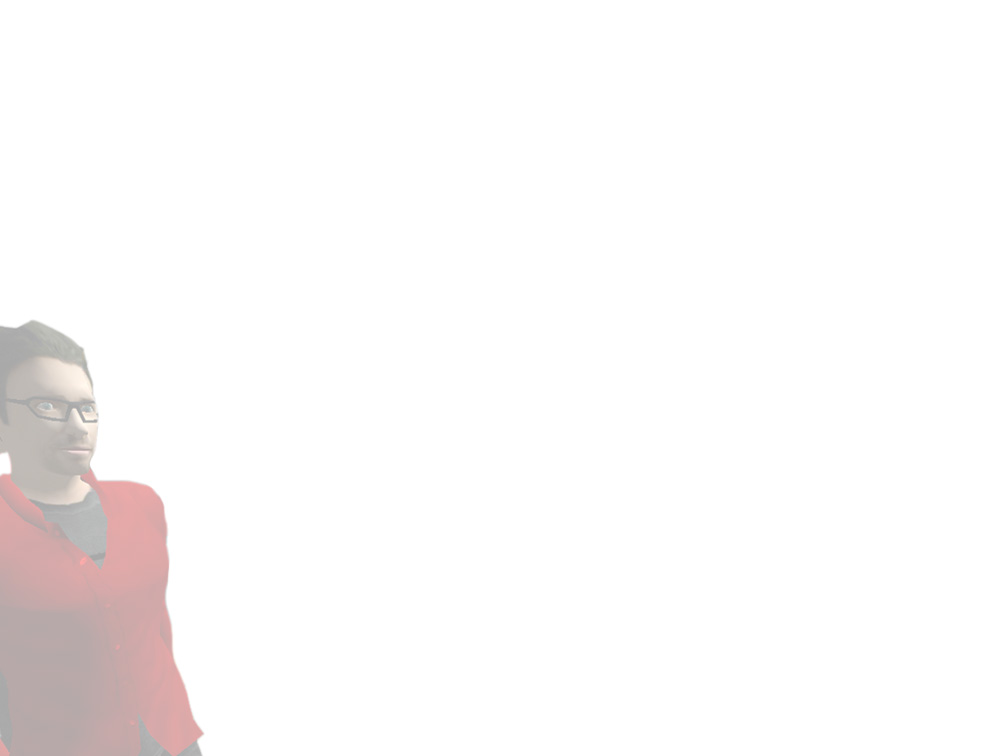
\includegraphics[width=\paperwidth,height=\paperheight]{Background2.jpg}}
	\begin{frame}
		\titlepage
	\end{frame}
	\usebackgroundtemplate{} % to remove the background picture from the start slide


	%\newcommand\tab[1][1cm]{\hspace*{#1}}
\graphicspath{{images/}{images/logos/}}
\begin{frame}{Unsere Aufgabe}
	\begin{center}
		\begin{itemize}
			\item Simulation des Festzuges in der Landshuter Innenstadt
			\item Menschen, Pferde und Kutschen sollen eingebunden werden
			\item Weitergabe der Ergebnisse
		\end{itemize}
	
\end{center}
	\underline{Simulations Tool:} $\underline{}$
	\begin{itemize}
		\item OpenVadere (Open Source Projekt) 
	\end{itemize}
\end{frame}

\begin{frame}{Sprint Ziele}
	\begin{center}
		\begin{itemize}
			\item US-2: Horse Modell:
			\begin{itemize}
				\item Unabhängiges Bewegungsmodell für das Pferd festlegen
			\end{itemize}
			\item US-7: Schnittstelle:
			\begin{itemize}
				\item Datenweitergabe an die Unity Gruppe
				\item Weitergabe der Rechenergebnisse an die CityGML Gruppe
			\end{itemize} 
			\item US-8: Landshuter Hochzeit (Teilszenario):
			\begin{itemize}
				\item Realität nah ein Teilszenario der Landshuter Hochzeit abbilden
			\end{itemize}
			\item US-5: Kutsche (Optional): 
				\begin{itemize}
				\item Erstellung einer Kutsche
			\end{itemize}
		\end{itemize}
	\end{center}
\end{frame}

\begin{frame}{Erreichte Ziele}
	\begin{center}
		\begin{itemize}
			\item \colorbox{green} {US-2: Horse Modell:}
			\begin{itemize}
				\item \colorbox{green} {Unabhängiges Bewegungsmodell für das Pferd fetlegen}
			\end{itemize}
			\item \colorbox{yellow} {US-7: Schnittstelle:}
			\begin{itemize}
				\item \colorbox{green} {Datenweitergabe an die Unity Gruppe}
				\item \colorbox{red}{Weitergabe der Rechenergebnis an die CityGML Gruppe}
			\end{itemize} 
		
			\item \colorbox{green} {US-8: Landshuter Hochzeit (Teilszenario):}
			\begin{itemize}
				\item \colorbox{green}{Realität nah ein Teilszenario der Landshuter Hochzeit abbilden}
			\end{itemize}
			\item \colorbox{green}{US-5: Kutsche (Optional):} 
			\begin{itemize}
				\item \colorbox{green}{Erstellung einer Kutsche}
			\end{itemize}
		\end{itemize}
	\end{center}
\end{frame}

\begin{frame}{Schwierigkeiten und Lösungen}
	\begin{itemize}
		\item Viele mögliche Ideen, wenig Kapazitäten
		 \begin{itemize}
			\item Festlegen fester User Stories, als Ziel 
			\item Leitung durch Scrum Master welche Task Priorität haben
		\end{itemize} 
		\item Verstreutes Team
			 \newline Treffen:
			 \begin{itemize}
			 	\item Donnerstags (Vorlesung)
			 	\item Sonntags(Online)
			 	\item Dienstags (Freiwillig HM)
			 \end{itemize} 
	\end{itemize}
\end{frame}

\begin{frame}{Ausblick}
	\begin{itemize}
		\item Komplette Simulation der Landshuter Hochzeit in viele Teilszenarien
		\item Weitergabe der Daten an die CityGML Gruppe
	\end{itemize}
\end{frame}

	%\newcommand\tab[1][1cm]{\hspace*{#1}}
\graphicspath{{images/}{images/logos/}}
\begin{frame}{Übersicht GUI}
	\begin{center}
		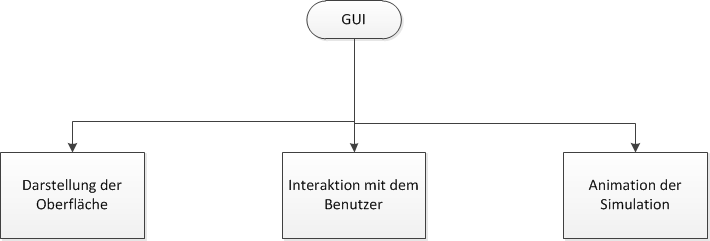
\includegraphics[width=710,height=241]{./model2.png}
	\end{center}
\end{frame}

\begin{frame}{Darstellung der Oberfläche}
	\begin{center}
		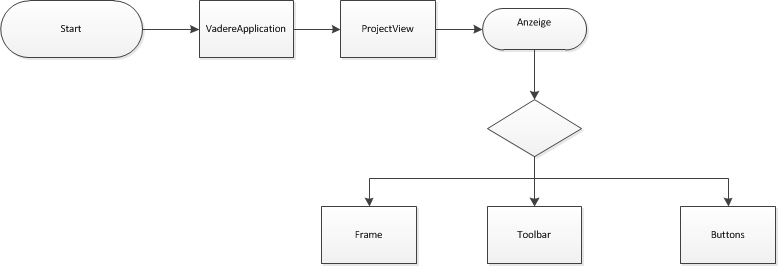
\includegraphics[width=778,height=266]{./model21.png}
	\end{center}
\end{frame}

\begin{frame}{Verwaltung der Actions}
	\begin{center}
		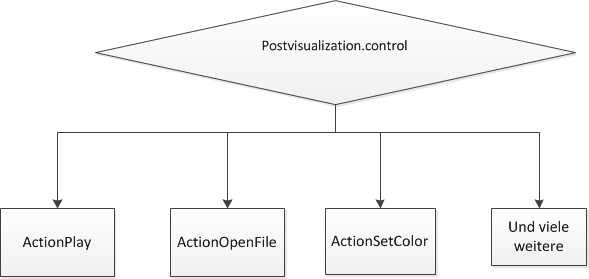
\includegraphics[width=589,height=279]{./model22a.png}
	\end{center}
\end{frame}


\begin{frame}{Verwaltung der Scenarios}
	\begin{center}
		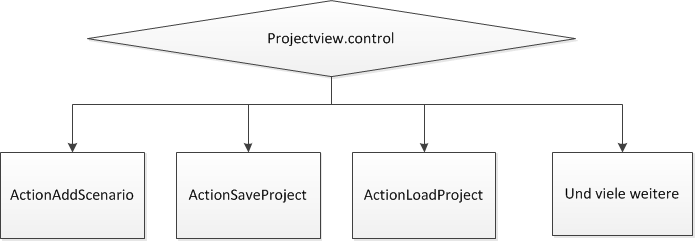
\includegraphics[width=695,height=241]{./model22b.png}
	\end{center}
\end{frame}


\begin{frame}{Zeichnen des Scenarios}
	\begin{center}
		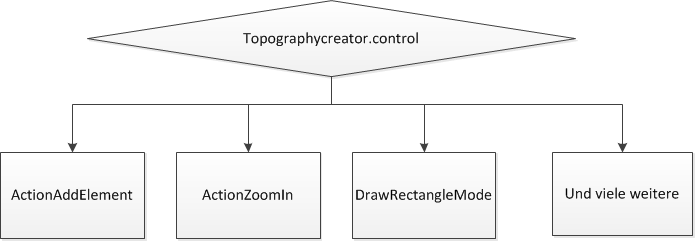
\includegraphics[width=695,height=241]{./model22c.png}
	\end{center}
\end{frame}


\begin{frame}{Animation der Simulation
	\begin{center}
		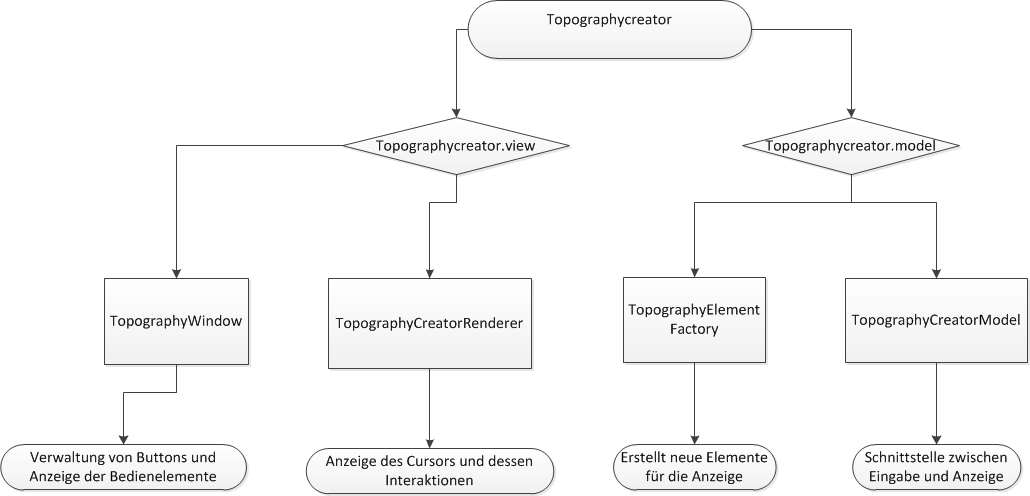
\includegraphics[width=1030,height=496]{./model23a.png}
	\end{center}
\end{frame}

\begin{frame}{Zeichnen der Grafiken}
	\begin{center}
		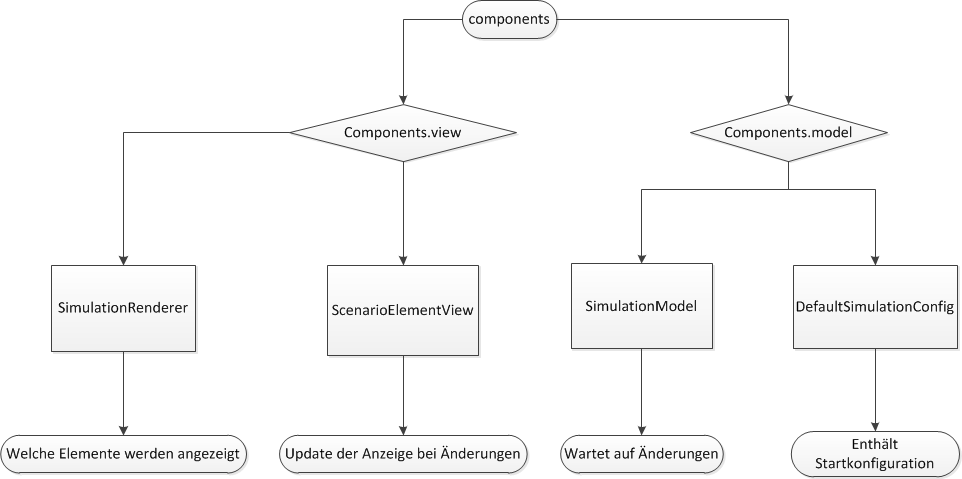
\includegraphics[width=962,height=479]{./model23b.png}
	\end{center}
\end{frame}


\begin{frame}{Button zu Horse}
	\begin{center}
		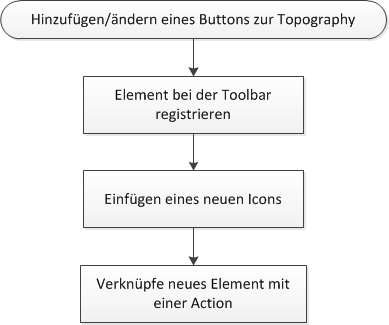
\includegraphics[width=389,height=325]{./model31.png}
	\end{center}
\end{frame}


\begin{frame}{Einbinden der Klasse Horse in GUI}
	\begin{center}
		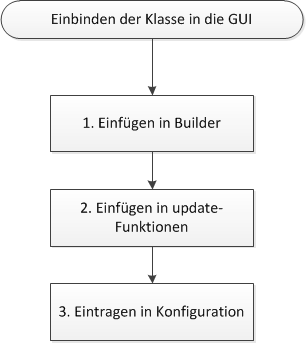
\includegraphics[width=306,height=343]{./model32a.png}
	\end{center}
\end{frame}


\begin{frame}{Einfügen in Builder}
	\begin{center}
		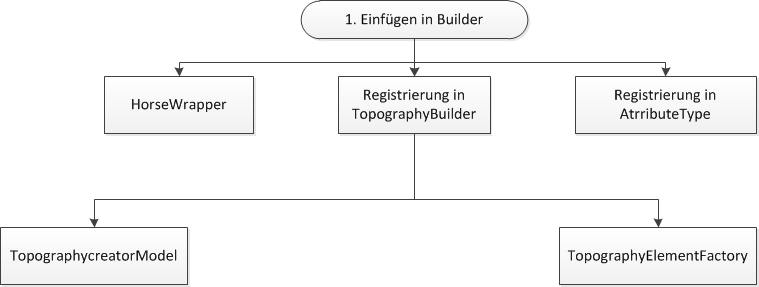
\includegraphics[width=759,height=287]{./model32b.png}
	\end{center}
\end{frame}

\begin{frame}{Einfügen in update - Funktionen}
	\begin{center}
		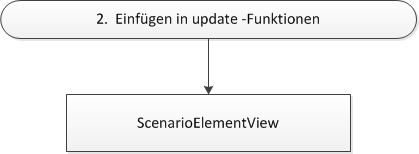
\includegraphics[width=419,height=154]{./model32c.png}
	\end{center}
\end{frame}

\begin{frame}{Eintragen in Konfiguration}
	\begin{center}
		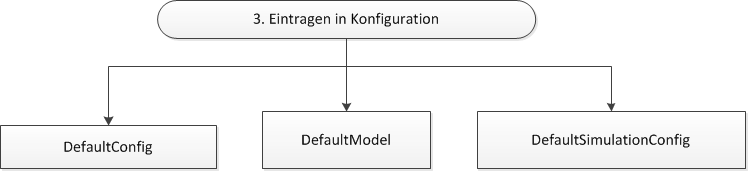
\includegraphics[width=748,height=171]{./model32d.png}
	\end{center}
\end{frame}



	\begin{frame}
	\begin{center}
		\Huge Daniel Jadanec
	\end{center}
\end{frame}

\begin{frame}
	 \begin{enumerate}
		 \item Mein Aufgabenbereich
		 \item Bisheriger Stand
		 \item Anforderung
		 \item Umsetzung
		 \item Ergebnis
		 \item Fazit
	\end{enumerate}
\end{frame}

\begin{frame}{Mein Aufgabenbereich}
	\begin{itemize}
		\item VR Trajectory Datei mit den Berechnungen von Vadere
		\item Bugfixes und Optimierung
		\item Bimodales Simulationsmodell
	\end{itemize}

	\begin{minipage}{0.4\textwidth}
		\begin{figure}
			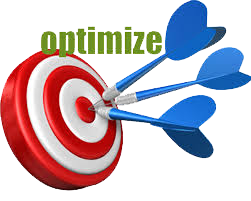
\includegraphics[width=\textwidth]{appendix/images/caricature/optimize.png}
		\end{figure}
	\end{minipage} \hfill
	\begin{minipage}{0.5\textwidth}
			\begin{figure}[H]
				
\includegraphics[width=\textwidth]{appendix/images/caricature/bugfixer.png}
			\end{figure}
	\end{minipage}
\end{frame}

\begin{frame}{Bisheriger Stand}
	\begin{itemize}
		\item Trajectory hatte keine Information über Agententypen
		\item Die Simulation lief nur mit einem Bewegungsmodell \cite{zarnitz-2015}
	\end{itemize}
\end{frame}

\begin{frame}{Anforderung}
	\begin{enumerate}
		\item VR Gruppe soll eine eigene Trajectory Datei bekommen
		\item Der Code soll für den letzten Sprint optimiert werden
		\item Mehrere Bewegungsmodelle sollen interagieren
	\end{enumerate}
\end{frame}

\begin{frame}{Umsetzung: UML Trajectory für VR}
	\begin{figure}
		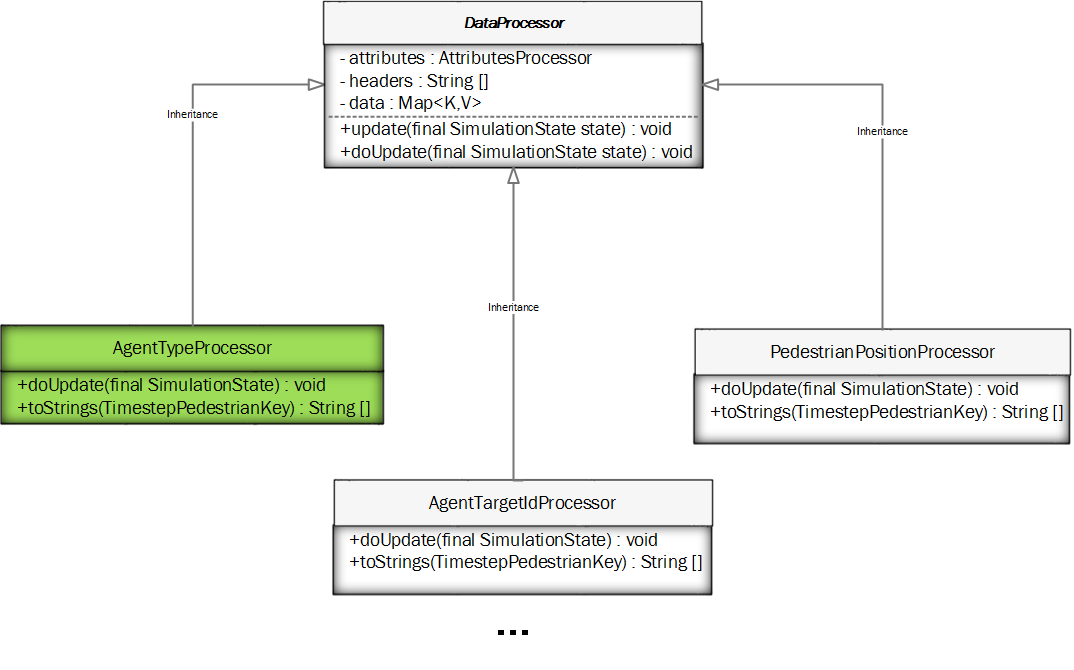
\includegraphics[width=\textwidth, keepaspectratio]{appendix/uml/OutputProcessor.png}
	\end{figure}
\end{frame}

\begin{frame}{Ergebnis: Trajectory für VR}
	\begin{minipage}{0.4\textwidth}
		\begin{itemize}
			\item Agent-Typ numerisch angegeben
			\item Leichte Ergänzung weiterer Prozessoren
			\item Datei exklusiv für die VR Gruppe und ihre Bedürfnisse angepasst
		\end{itemize}
	\end{minipage} \hfill
	\begin{minipage}{0.5\textwidth}
			\begin{figure}[H]
				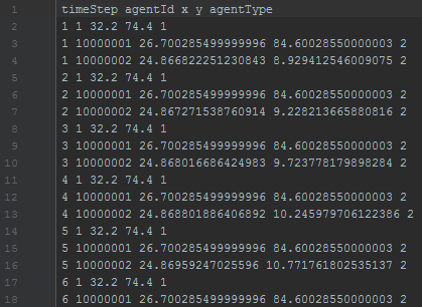
\includegraphics[width=\textwidth]{appendix/images/Trajectory.png}
			\end{figure}
	\end{minipage}
\end{frame}

\begin{frame}{Umsetzung: Bimodales Modell}
	\begin{figure}
		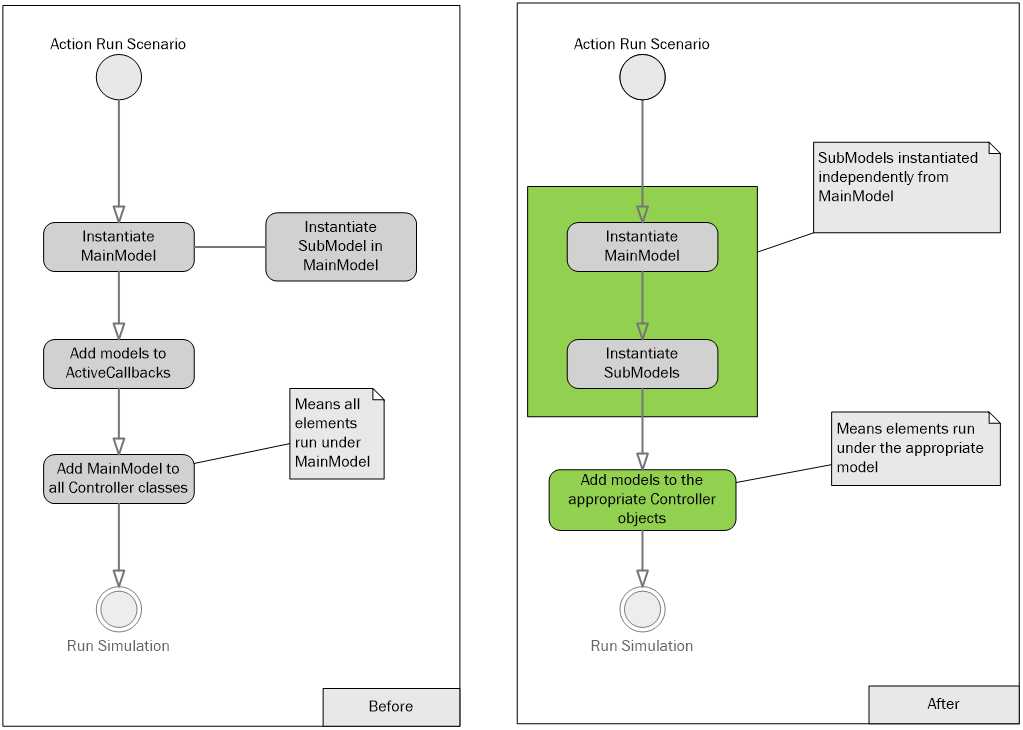
\includegraphics[width=\textwidth, height=0.8\textwidth, keepaspectratio]{appendix/uml/MotionModels.png}
	\end{figure}
\end{frame}

\begin{frame}{Änderung der Json Konfiguration}
	\begin{figure}
		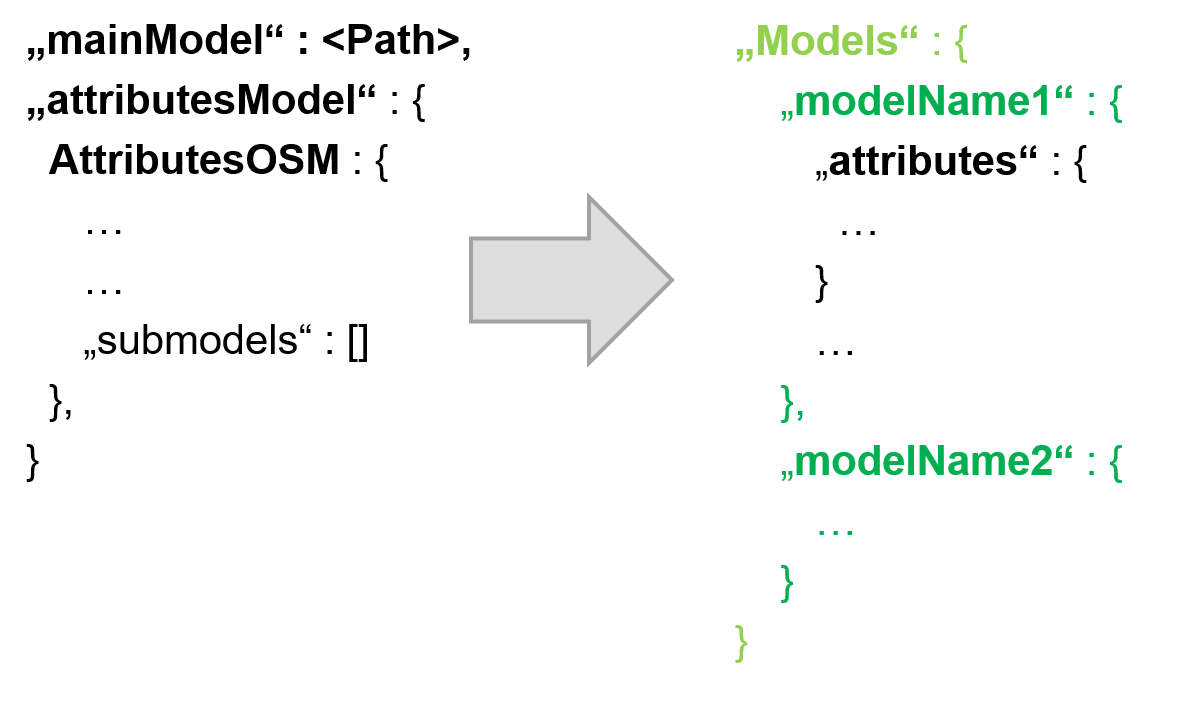
\includegraphics[width=\textwidth, height=0.8\textwidth, keepaspectratio]{appendix/images/JsonChange.png}
	\end{figure}
\end{frame}

\begin{frame}{Zweck der Änderung}
	\begin{itemize}
		\item	Mehrere Bewegungsmodelle erhalten nun Konfigurationsdaten
		\item Festlegen der Szenario Elemente, die mit dem Modell laufen sollen
		\item Der SubModel Knoten kann weitergeführt werden, nun aber als tatsächliches Untermodell
	\end{itemize}
\end{frame}

\begin{frame}{Ergebnis: Bimodales Modell}
	\begin{figure}
		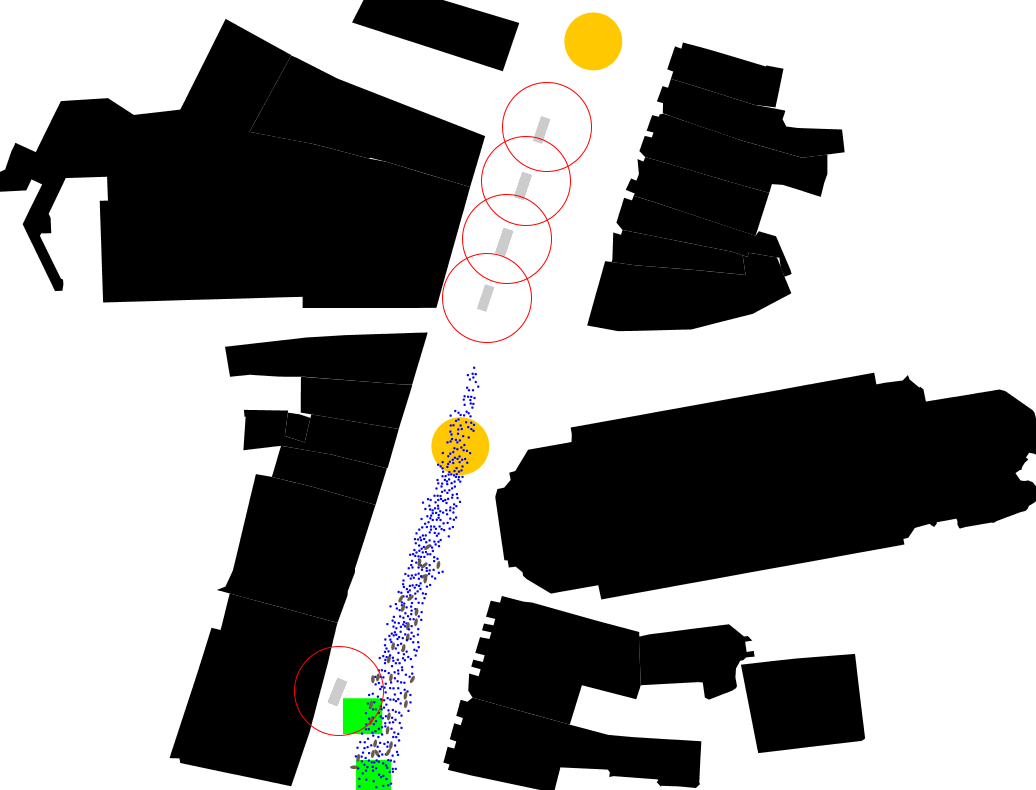
\includegraphics[width=\textwidth, height=0.7\textwidth, keepaspectratio]{appendix/images/landshutbimodal.png}
	\end{figure}
\end{frame}

\begin{frame}{Fazit}
	\par{Positiv:}
	\begin{itemize}
		\item Aufgabenzuweisung und Taskerstellung ging sehr schnell
		\item Scrum Master hielt das „Böse“ von uns fern
		\item Gut strukturierter Sprint mit festgelegten Meetings
	\end{itemize}

	\par{Ausbaufähig:}
	\begin{itemize}
		\item Gewicht/Schwierigkeit eines Tasks
		\item Mehr Tests sollten geschrieben werden
		\item Engere Zusammenarbeit mit den anderen Teams. Für den letzten Sprint unumgänglich!
	\end{itemize}

	\par{ Selbsteinschätzung: 23 \% }
\end{frame}

	%\newChapterSlide{Andrei Yauseyenka}{Vortrag, Icon, Galerie}{}{20}{2}
\setbeamercovered{invisible}

%
%% ----- FRAME 1 -----
%

\begin{frame}{Vortrag}

Vortrag über Studium mit Schwerpunkt auf dem Modelierungsseminar

\pause

\textbf{Rückfragen}

	\begin{itemize}

		\item Bewegung von Gruppen
		\item Unterschiedliche Geschwindigkeiten
		\item Unterschiedliche Anfagszeiten (Bier noch halb voll)
		\pause
	\end{itemize}

\textbf{Rückmeldung der Anwesenden}
	\begin{itemize}

		\item Cardboard als Hauptattraktion
		\item Kamera zu niedrig
		\item Interesse an App
		\item Bierzeltgefühl

	\end{itemize}


\end{frame}

\begin{frame}{Icon}

	\begin{minipage}{0.50\textwidth}
			\includegraphics[width=\textwidth]{pres_pics/hm_icon.jpg}
	\end{minipage} \hfill
	\begin{minipage}{0.48\textwidth}
		\begin{itemize}
			\item Schlicht
			\item Quadratisch
			\item Transparenter Hintergrund
		\end{itemize}
	\end{minipage}

\end{frame}

\begin{frame}{Icon}

	\begin{minipage}{0.50\textwidth}
		\includegraphics[width=\textwidth]{pres_pics/hm_icon.jpg}
	\end{minipage} \hfill
	\begin{minipage}{0.48\textwidth}
		\includegraphics[width=\textwidth]{pres_pics/hm_icon2.png}
	\end{minipage}

\end{frame}

\begin{frame}{Galerie}

	\includegraphics[width=\textwidth]{pres_pics/galerie.png}
	\begin{itemize}
		\item 66 Tische, 132 Bänke
		\item 660 Personen, bei nur 2 Treppen
		\item Rechnung mit 300 Personen pro Treppe
	\end{itemize}

\end{frame}

\begin{frame}{Galerie}

		\begin{minipage}{0.50\textwidth}
		\includegraphics[width=\textwidth]{pres_pics/5p_vorher.png}
	\end{minipage} \hfill
	\begin{minipage}{0.48\textwidth}
		\includegraphics[width=1.04\textwidth]{pres_pics/mitGalerie.png}
	\end{minipage}

\end{frame}

\begin{frame}{Galerie}

		\begin{minipage}{0.50\textwidth}
		\includegraphics[width=\textwidth]{pres_pics/ohneGaleriePersonenstrom.png}
	\end{minipage} \hfill
	\begin{minipage}{0.48\textwidth}
		\includegraphics[width=1.04\textwidth]{pres_pics/GaleriePersonenstrom.png}
	\end{minipage}

\end{frame}

\begin{frame}{Galerie}

		\begin{minipage}{0.50\textwidth}
		\includegraphics[width=\textwidth]{pres_pics/GalerieEnde.png}
	\end{minipage} \hfill
	\begin{minipage}{0.48\textwidth}
		\begin{itemize}
			\item Zelt schon evakuiert
			\item Galerie aber noch nicht
			\item Evakuierungszeit eine Minute länger
		\end{itemize}
	\end{minipage}

\end{frame}

\begin{frame}{Kamerafashrt}


		\includegraphics[height=0.8\textheight]{pres_pics/KamerafahrtPositionen.png}


\end{frame}

\setbeamercovered{transparent}

	%\graphicspath{{images/}{images/logos/}}

\begin{frame}{Meine Tätigkeiten}
	\begin{itemize}
		\item Scrum Master
			\subitem Koordination
			\subitem Ansprechpartner
			\subitem ....
		\item Einarbeiten in den Simulator
			\begin{itemize}
				\item Verstehen wie Simulationen ablaufen
				\item Was muss angepasst werden für neue Agenten
			\end{itemize}
		\item Erweitern des Simulators um Horse
	\end{itemize}
\end{frame}  

\begin{frame}{Ablauf der Simulation}
	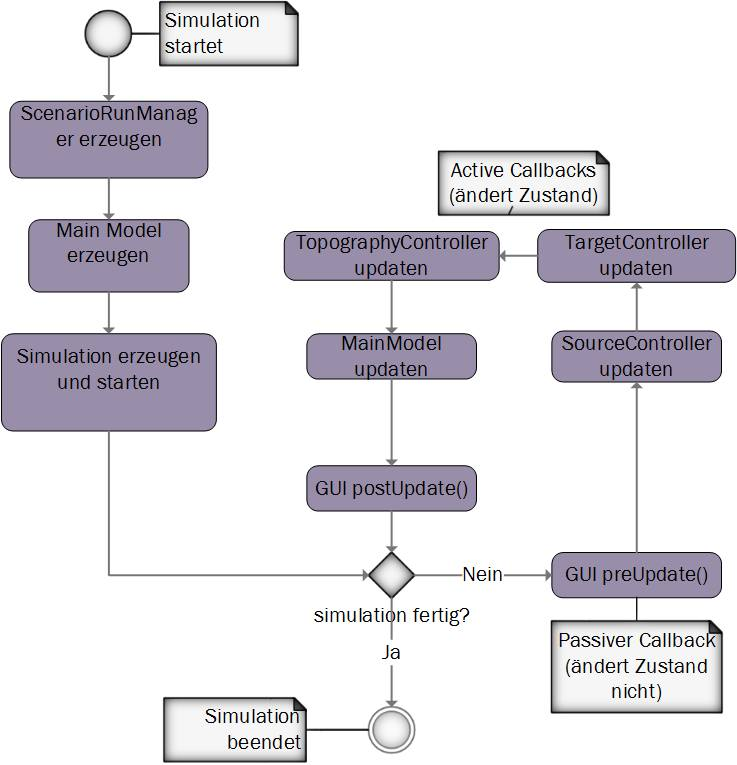
\includegraphics[width=250,height=240]{./simul.png}
\end{frame}

\begin{frame}{Fazit}
	\begin{itemize}
		\item 	\underline{Fand ich gut:} \newline $\underline{}$
			\begin{itemize}
				\item Gelegenheit an einem größeren Projekt zu arbeiten
				\item Gute Zusammenarbeit (skype und trello)
			\end{itemize}
		\newline
		\item \underline{Kann besser sein:} \newline $\underline{}$
			\begin{itemize}
				\item Einbezug in aktuelle Änderungen des Codes
				\item Regelmäßiger Treffen \newline
			\end{itemize}
		\item \underline{Anteil Schätzung:} $\underline{}$ \tab 19\%
	\end{itemize}
\end{frame}
	%\begin{frame}{Meine Aufgaben}
	\begin{itemize}
		\item Einarbeiten in das Optimal Steps Model
		\item Einbinden der Horse Klasse ins OSM
		\item Erstellen eines Testszenarios 
	\end{itemize}
\end{frame}

\begin{frame}{Optimal Steps Model}
	\begin{itemize}
		\item Nutzenfunktion
		\item Optimization
		\item Update Schemes
	\end{itemize}
\end{frame}

\begin{frame}{Implementierung OSM}
	\begin{figure}
		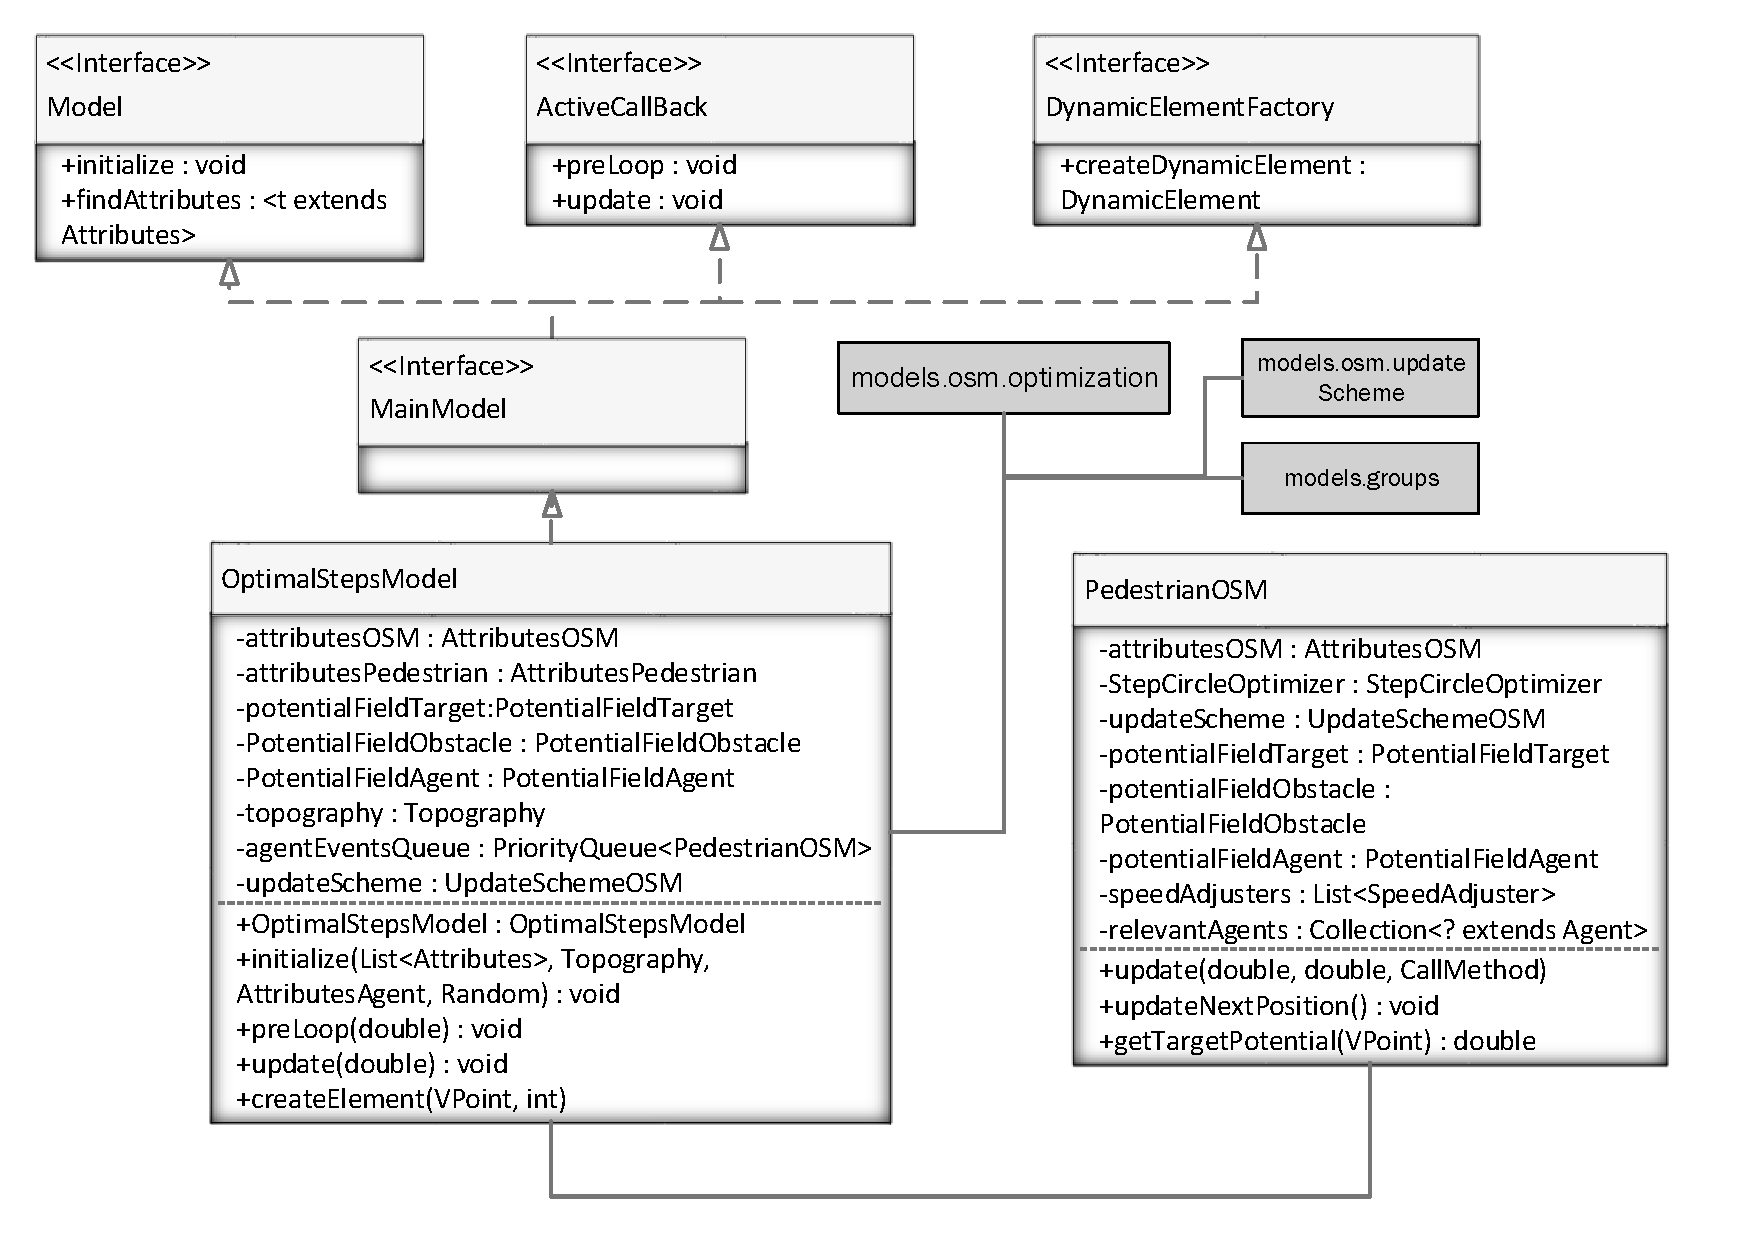
\includegraphics[width=\textwidth, keepaspectratio]{appendix/uml/OSM-vorher.pdf}
	\end{figure}
\end{frame}

\begin{frame}{Implementierung HorseOSM}
	\begin{figure}
		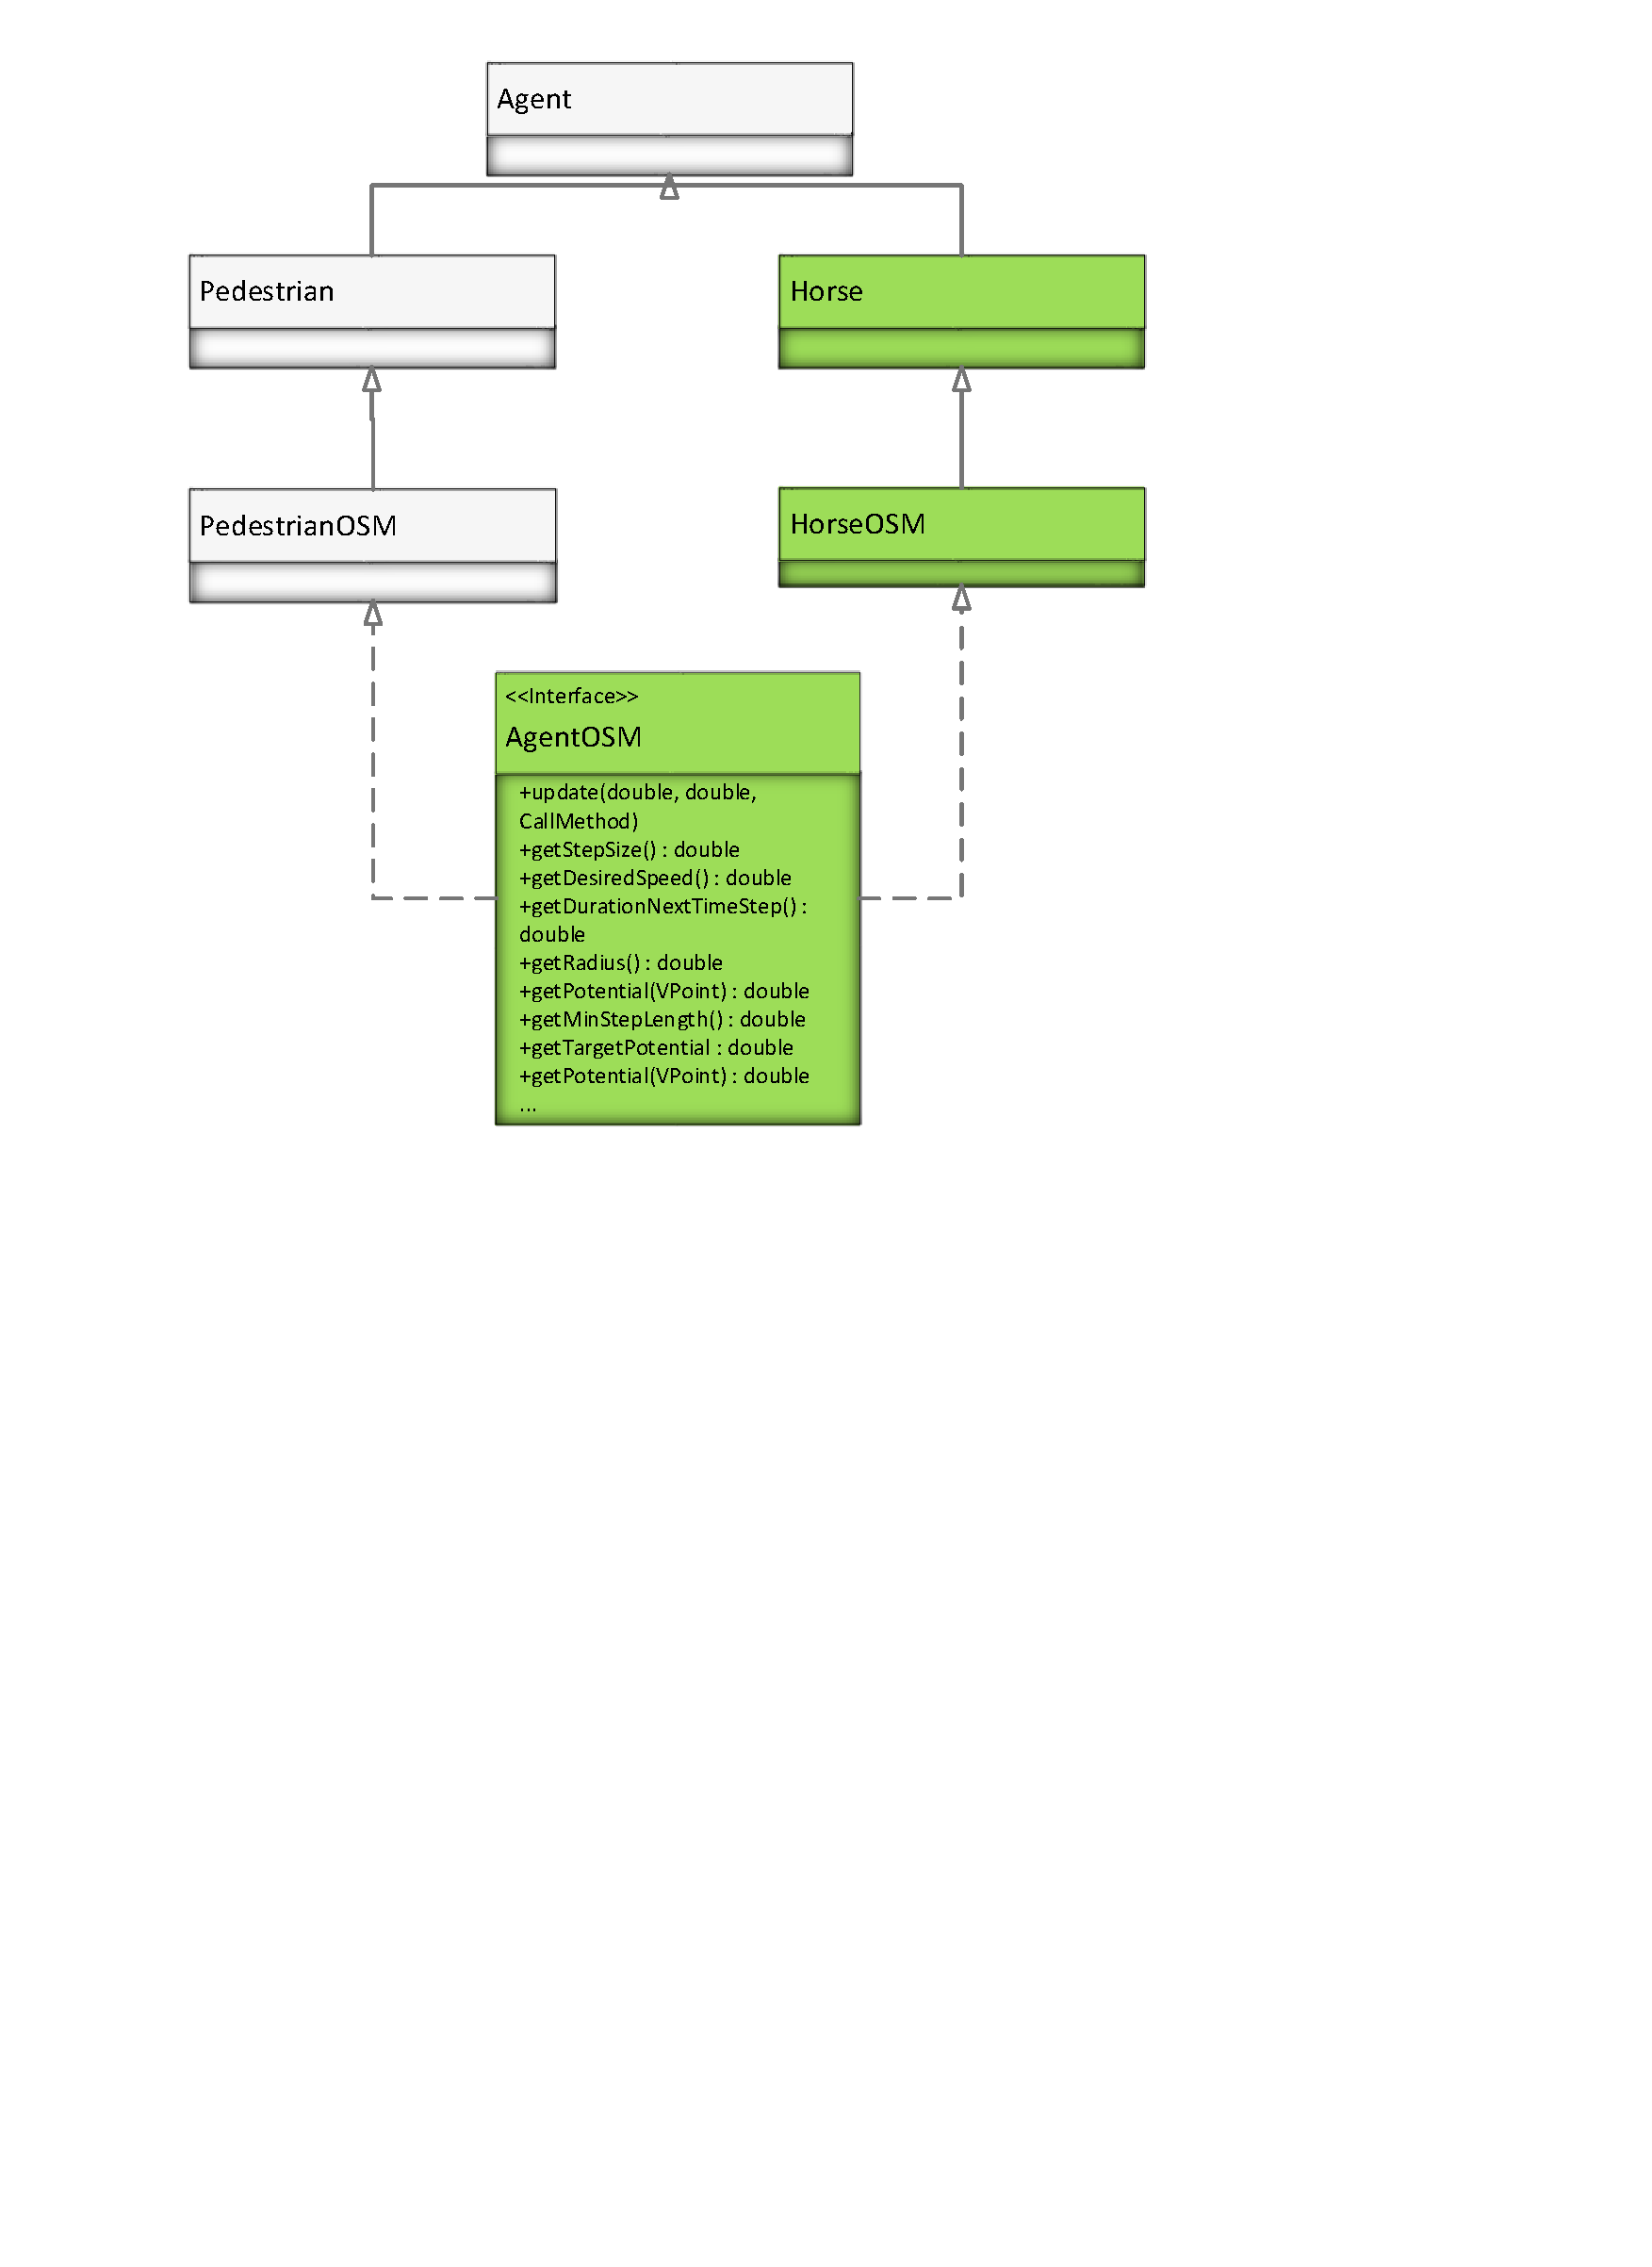
\includegraphics[width=\textwidth, keepaspectratio]{appendix/uml/OSM-nachher.pdf}
	\end{figure}
\end{frame}

\begin{frame}{Ein Schritt im OSM}
	\begin{figure}
		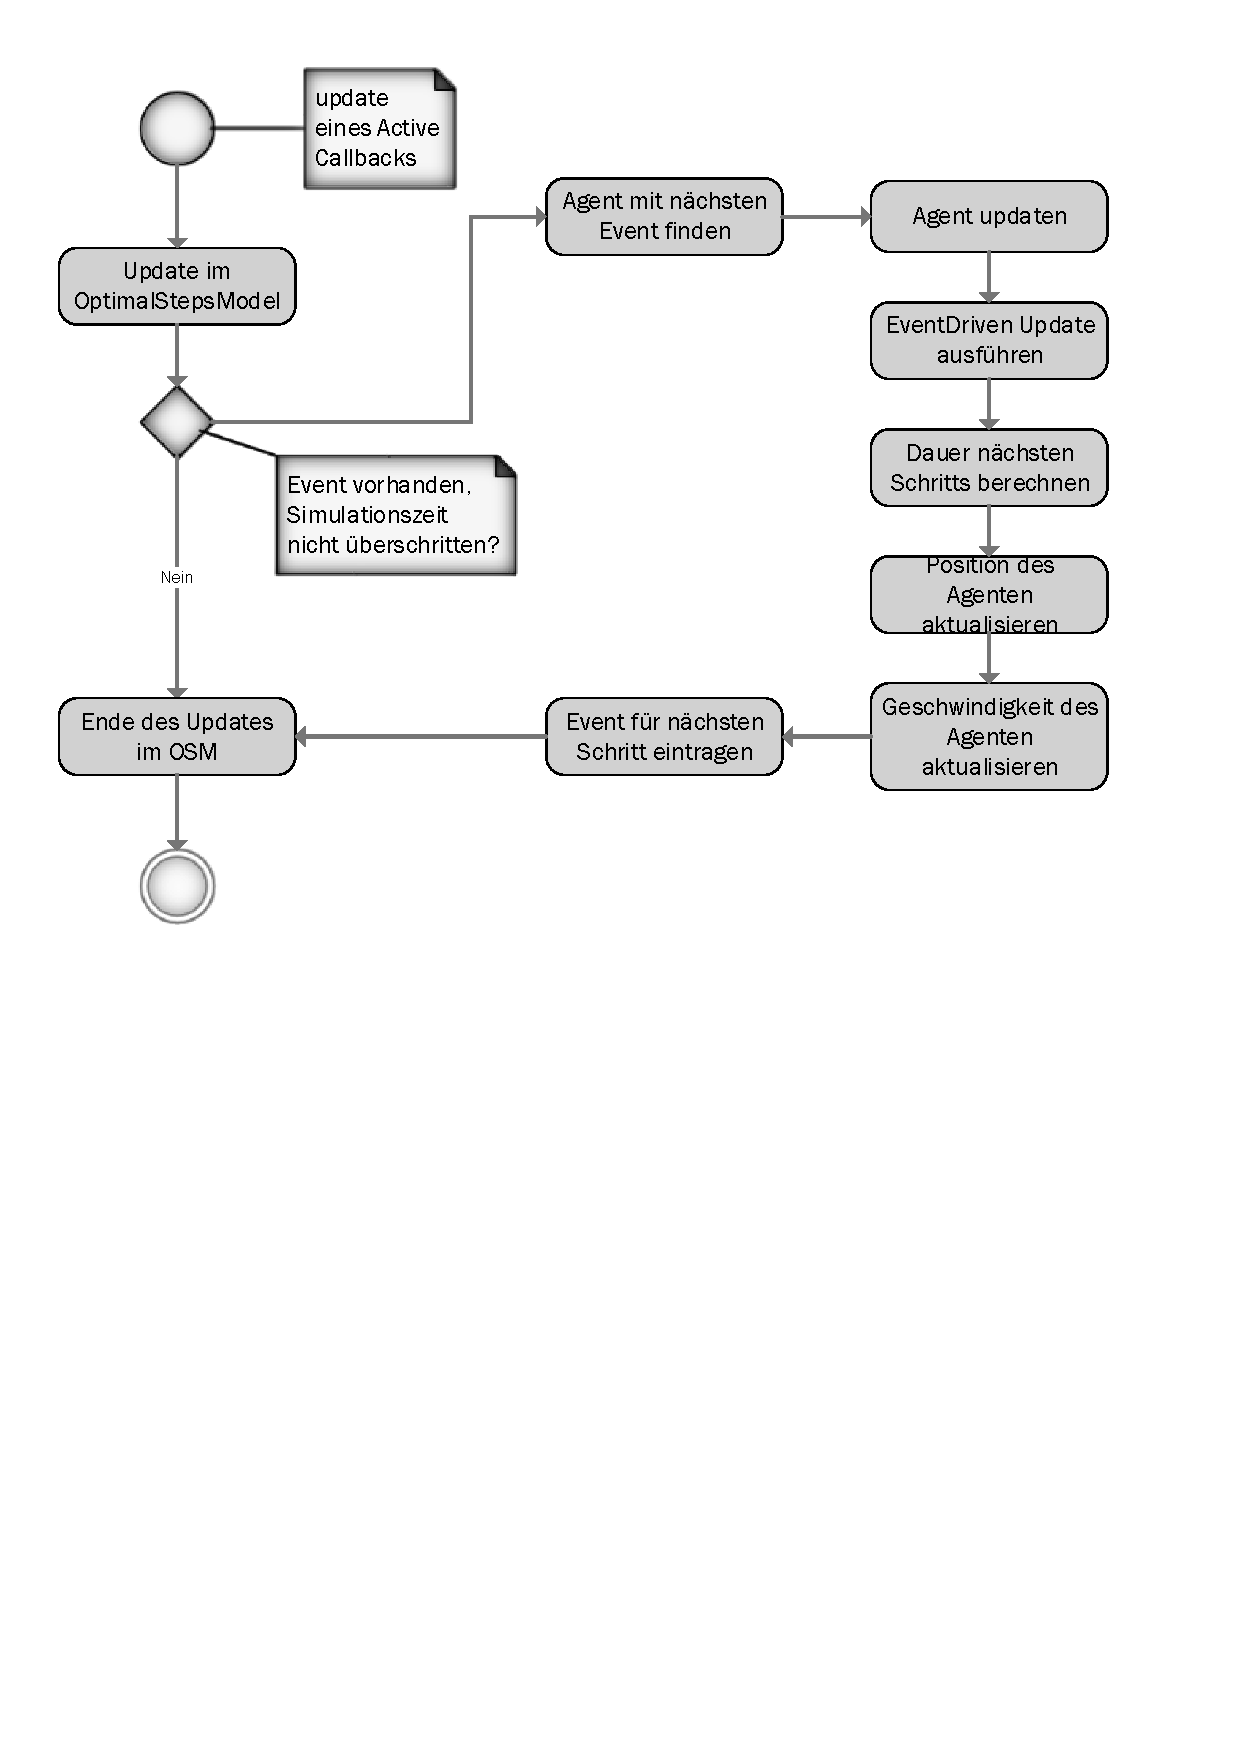
\includegraphics[width=\textwidth, keepaspectratio]{appendix/uml/EventDrivenUpdate.pdf}
	\end{figure}
\end{frame}

\begin{frame}{Fazit}
	Schwierigkeiten:
	\begin{itemize}
		\item Meine Arbeitszeiten
	\end{itemize}
	Fand ich gut:
	\begin{itemize}
		\item Organisation durch Trello, Skype
		\item Arbeitsaufteilung
		\item gutes Klima
		\item Anteil 19\%
	\end{itemize}
\end{frame}


	%\include{presentations/outro}


	\begin{frame}[allowframebreaks]{Quellen}
		\setbeamertemplate{bibliography item}[text]
		\bibliographystyle{plain}
		\bibliography{Literature}
	\end{frame}

%%%%%%%%%%%%%%%%%%%%%%%%%%%%%%%%%%%%%%%%%%%%%%%%%%%%%%

\end{document}
